%\documentclass{article}
%\usepackage[a4paper, total={6in, 8in}]{geometry}
%\documentclass[reprint,amsmath,amssymb,rmp,onecolumn,notitlepage,11pt]{revtex4-1}
\documentclass[
reprint,
twocolumn,
%preprint
%onecolumn,
amsmath,amssymb,superscriptaddress,aps,
pre]{revtex4-1}
\usepackage[utf8]{inputenc}
%\usepackage{authblk}
%\usepackage{natbib}
\usepackage[normalem]{ulem}
\usepackage{graphicx}
\usepackage{hyperref}
\usepackage{xcolor}
\newcommand{\red}[1]{\textcolor{red!80!black}{#1}}
\newcommand{\blue}[1]{\textcolor{blue!80!black}{#1}}
\newcommand{\green}[1]{\textcolor{green!70!black}{#1}}
\newcommand{\gray}[1]{\textcolor{gray!80!black}{#1}}
\usepackage{mathtools}
\DeclarePairedDelimiter{\evdel}{\langle}{\rangle}
\usepackage[colorinlistoftodos]{todonotes}

\begin{document}
\title{Chain separation distribution in protein contact networks}
\title{Theoretical approximation of chain separation distribution in protein contact networks}
\title{Theory of chain separation distributions gives insights in real protein contact networks}
%\title{}
\author{Nora Molkenthin}
\affiliation{Potsdam Institut für Klimafolgenforschung}
\affiliation{Center for Advancing Electronics Dresden (cfaed), Technical University of Dresden}
\author{Steffen Mühle}
\affiliation{Uni Göttingen, 37077 Göttingen, Germany}
\author{Antonia S J S Mey}
\email[Electronic Address: ]{antonia.mey@ed.ac.uk}
\affiliation{EaStCHEM School of Chemistry, University of Edinburgh, Edinburgh, United Kingdom}
%\author{Marc Timme}
% \affiliation{Network Dynamics, Max Planck Institute for Dynamics and Self-Organization (MPIDS), 37077 Göttingen, Germany}
% \affiliation{Chair for Network Dynamics, Institute for Theoretical Physics and Center for Advancing Electronics Dresden (cfaed), Technical University of Dresden, 01069 Dresden}

\begin{abstract}
The mechanisms by which the folded structures of proteins are determined has long been one of the key mysteries of Biophysics. Here we approach the problem from a network ensemble perspective, analyzing the relative frequencies with which residues at different distances along the chain come into contact. We define and analyze the residue distance distribution for measured protein structures and structures resulting from a geometrically constrained random interaction model and find that the distributions are compatible. We furthermore derive an analytic approximation for the two dimensional analog of the model and find this approximation to also describe the distribution. We therefore propose the conclusion that the approximate power-law behaviour of the residue distance distribution is largely caused by geometric constraints of chains rather than specifics of protein sequences.
%The distribution of chain separations of interacting amino acids in proteins roughly follows a power law. Here we show, analytically and in simulations, that a geometrical stochastic model of folding chains can explain this behaviour. 
\end{abstract}
\maketitle

\section*{Introduction}
Proteins, the molecular machines of every living organism perform vital tasks required for life to persist, ranging from transport (e.g. hemoglobin), signal transduction (e.g. rhodopsin), immune responses (e.g. antibodies), and hormonal regulation (e.g. insulin)~\cite{something}. All natural proteins are made up of 20 different amino acids which dictate the three dimensional conformations the proteins adopt in order to function~\cite{stuff}. One way of looking at the functional forms of proteins and classifying their structural properties is by looking at protein residue or contact networks~\cite{Vendruscolo2002,DiPaola2013,Estrada2011}. Protein Contact Networks (PCN), have shown promise in understanding protein folding patterns as well as revealing allosteric communication pathways~\cite{https://pubs.acs.org/doi/10.1021/acs.jcim.9b00320, and others}. 
From a physicist perspective it is interesting to understand the emergent behaviour in protein structure from PCNs, by investigating common network measures and their behaviour for PCNs. For example Bartoli et al.~\cite{bartoli2008effect} build a model in which they assume that proteins have a residue distance distribution that follows $\frac{1}{\ell}$, where $\ell$ is the separation of two connected amino acids along the backbone chain as the simplest implementation of a connection probability, that decreases with the distance along the sequence. However, they do not provide a quantitative explanation for this assumption. 

Here, we show how a simple geometrical model can reproduce this heuristically found behaviour well, even providing a simple analytical approximation. The analytical approximation and geometrical model build on the idea that inherently geometrical objects, such as amino acids, imply that any resulting PCN network ensemble modelling them has to be spatially embedded~\cite{molkenthin2016scaling, molkenthin2020self}. 
Different approaches have been used in the past for geometrical models describing protein folding, some of which derived characteristics of the secondary structure from constraints on bond and torsion angles~\cite{maybe cite Flory stuff here as well?,Danielsson2010,Molkenthin2011} and others focused on the formation mechanisms of the tertiary structure~\cite{molkenthin2016scaling, molkenthin2020self}. 

Based on such considerations, the network formation process, repeatedly connects random pairs of units, without causing any intersections along the chain ~\cite{molkenthin2016scaling}. Such a model can now be used to investigate the emergent behaviour of residue distance distributions as used heuristically by Bartoli et al.~\cite{bartoli2008effect}. To this end, we define and analyze the residue distance distributions $P(s)$ that emerge from the geometric model, where the \emph{residue distance} $s$ of a link is defined as the distance of the two end units along the original chain.
This is then compared to the residue distance distribution extracted from protein contact networks generated from protein data bank data. 

We find that, despite the highly simplified model, the generated residue distance distribution is in agreement with the one observed in networks generated from PDB data and roughly consistent with the heuristic $1/s$ finding. The analytical approximation provides a correction term on top of the $1/s$ heuristic.


\section*{Protein Residue Networks and their synthetic counterparts}
The complex interaction pattern between the amino acids in a protein can be very naturally expressed as a network, in which each amino acid is represented by a node and spatial proximity is encoded as a link. Whenever two central $C_\alpha$ atoms are closer together than a threshold $d_c$, they are connected. These connections are encoded in the adjacency matrix of the folded protein, which is the binary matrix
\begin{equation}
  A^{\textsf{PDB}}_{ij}=
  \begin{cases}
   0, & \text{ if } d_{i,j}>d_c \text{ or } i=j\\
      1, & \text{ if } d_{i,j}\leq d_c .
      \end{cases}
    \label{eq:aij}
\end{equation}
Adjacency matrices are commonly used to describe networks and in this case represent the PCN.

The underlying formation mechanisms of individual protein folds are incredibly complex and depend on the surrounding solvent as well as the specific amino acid sequence and their quantum-mechanical interactions. Here we want to study the ensemble of all proteins, however, and will thus "average" over such specifics.

Based on the basic assumption that amino acids are objects in space, that can not overlap indefinitely, we introduced a model in \cite{molkenthin2020self} starting from a chain of identical spheres, each in contact only with the neighbours it is connected to. Then additional connections form by randomly selecting two spheres and moving them towards each other until they touch, the new links formed that way can not be broken in later steps and function as constraints on subsequent links. If contact of the two selected spheres is geometrically impossible without breaking previously made connections or leading to overlaps of any spheres, the link is not made and taken out of the pool of possible connections. This process is repeated until no more links can be formed without violating the geometric constraints.

In \cite{molkenthin2016scaling}, we have introduced a simplified, two-dimensional version of this model, which starts from a closed chain of $N$ unit discs and subsequently adds links, such that connected discs touch, yet no discs intersect. The advantage of this model is, that it can be approximated by a purely topological simplification, which can be treated analytically.

The topological constraints in the resulting network model are:
(a) New links always form between two units that are part of the same face of the graph (region enclosed by a cycle in the network). This prevents the overlapping of discs. (b) No links form across the outer face. This prevents the enclosure of a unit by less than six other units (which is geometrically impossible) such that. (c) The maximum degree of each unit is six, as six is the maximum number of unit discs, one central unit disc can touch. (d) Once connected by a link, pairs of units do not disconnect.

\section*{Analytic approximation}
Here we want to analytically approximate the residue distance distribution for the simplified 2D model, that is the separation along the backbone chain of two nodes connected by a link, as illustrated in Fig~\ref{fig:schematic}~a).

\begin{figure}[h]
    \centering
    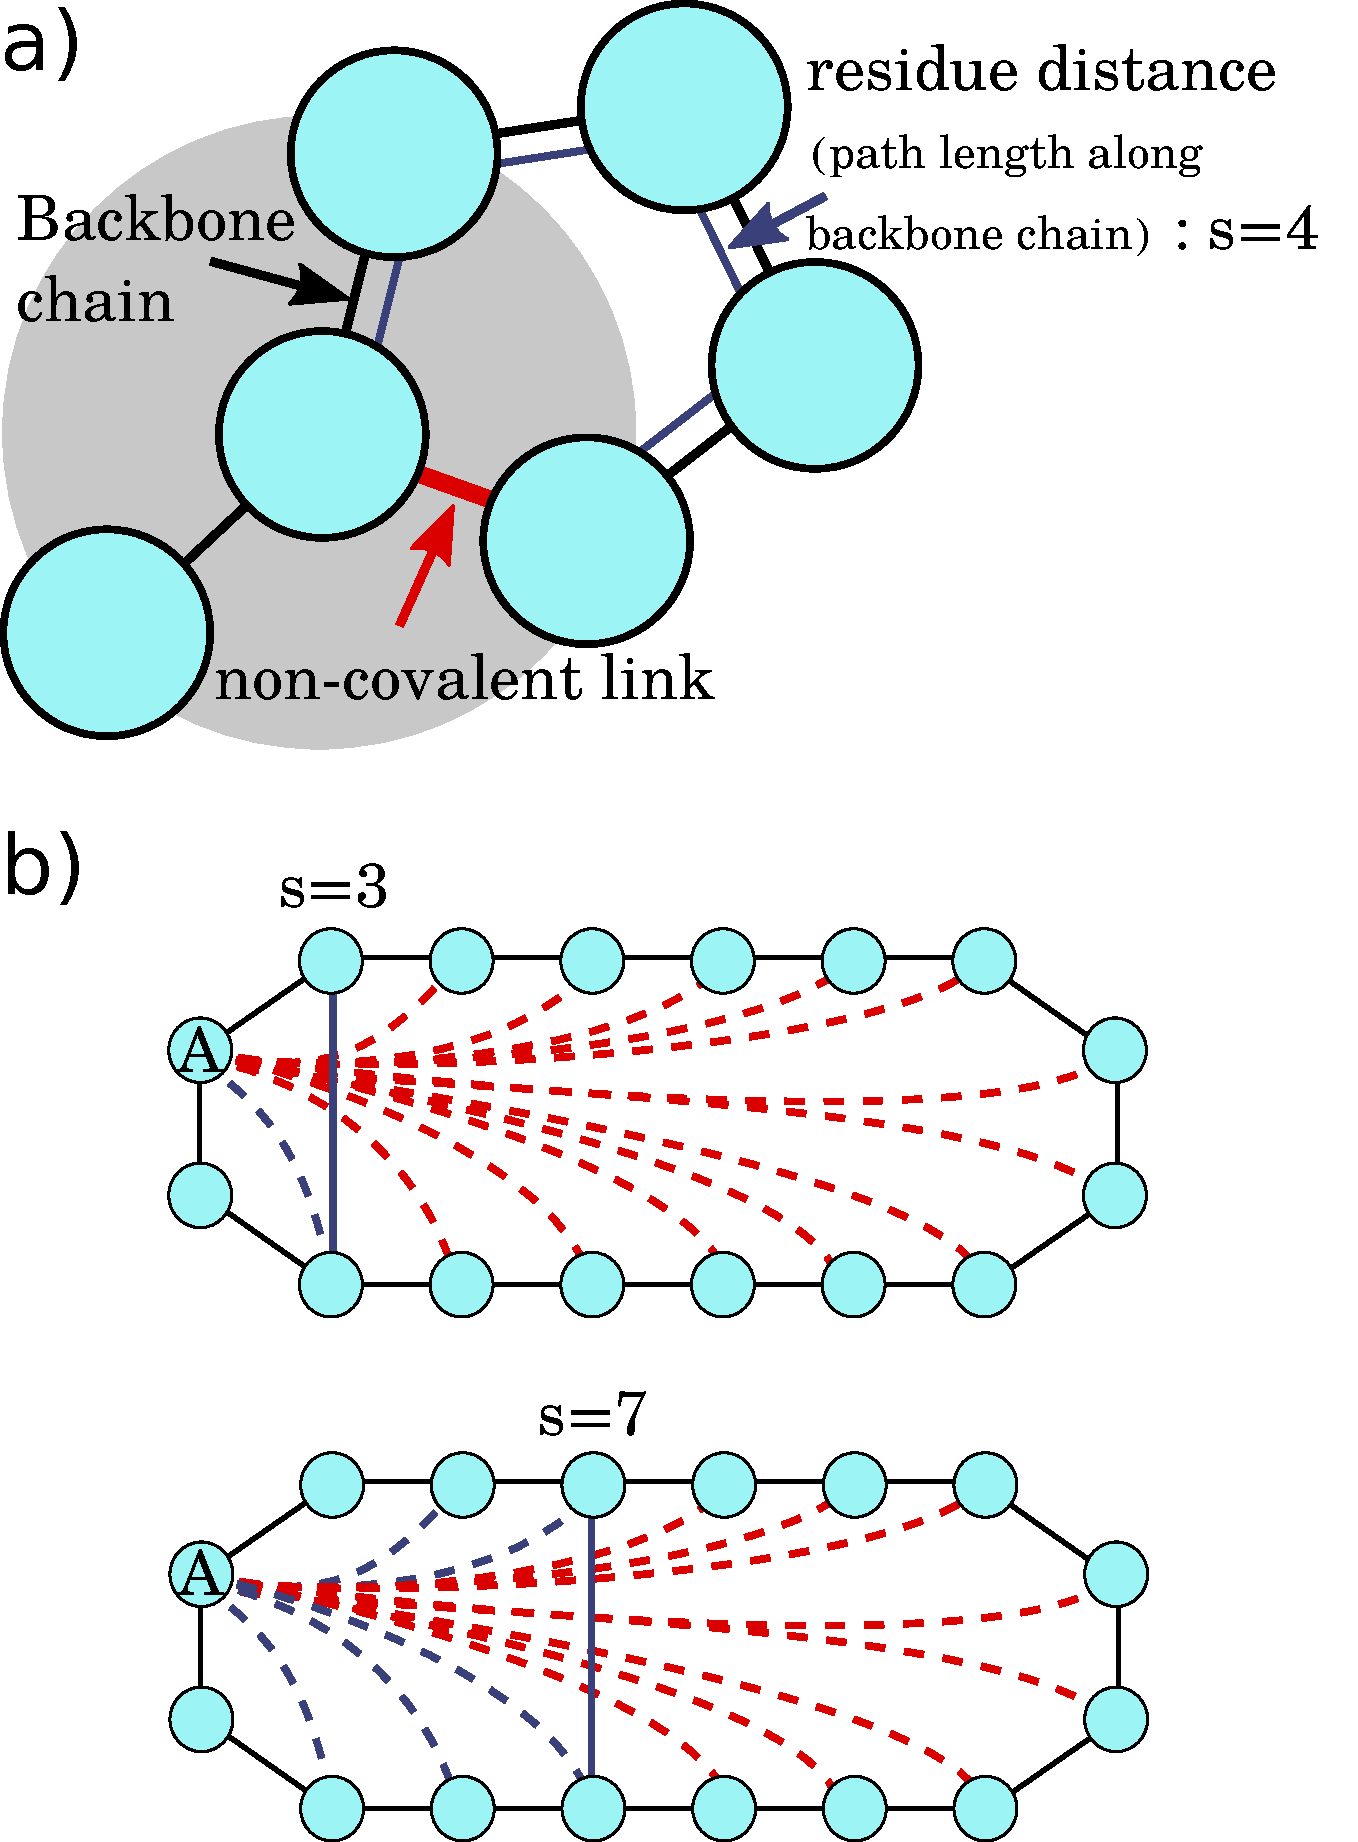
\includegraphics[width=0.7\columnwidth]{figures/Fig1/Fig1.pdf}
    \caption{a) The residue distance distribution is defined as the separation along the chain (blue) of two connected units (red). b) The solid blue link prohibits some connections from node $A$ (dotted red), while others are still permitted (dotted blue). Counting all newly excluded links, we find that a link of length $k$ prohibits $2(l-1)$ links of length $l$ up to a maximum of $k$ and $2(k-1)$ links of length $k$ or more.}
    \label{fig:schematic}
\end{figure}

Let us start by introducing the auxiliary variable $F(s)$, defined to be the number of possible links with a residue distance of $s$. Before any links are added all residue distances are equally likely, as there are $N$ possibilities of making a link of each separation $s$ with $2\leq s < N/2$.

As we add more links, not only are links taken out of this pool, because they have already been realized, each existing link can also geometrically prohibit other connections. Adding a link of length $s_1$ prohibits $2(s-1)$ links of length $s<s_1$ and $2(s_1-1)$ links of length $s>s_1$ (see Fig.~\ref{fig:schematic}~b). To find the expected number of links still available in subsequent stops, we average over all possible residue distances $s_1$ of the first link added.

The expected distribution of possible links after one step is given thus by the average over available link pools taken over all possible lengths of the initial link
\begin{equation}
    F_1(s)= \frac{1}{N/2-2} \sum_{s_1=2}^{N/2} { \begin{cases}
    N-2(s-1) \text{ , for } s<s_1\\
    N-2(s_1 -1)\text{ , for } s\geq s_1
    \end{cases}}.
\end{equation}
Here we denote the size of the pool of available links after $i$ links have been added $F_i(s)$.

In subsequent steps we get the same reduction but starting from the pool $F_{k-1}(s)$ of the step before rather than the full $N$ links for each length. The reduction also needs to be multiplied by a factor 
\begin{equation}
    P_k(s)=\frac{F_k(s)}{C_k},
    \label{eq.Pk}
\end{equation}
with $C_k=\sum_{s=2}^{N/2}F^k(s)$, to only remove links that are still in the pool. This leads to the recursion
\begin{align}
    F_k(s)&= \frac{1}{N/2-2} \nonumber \\
    &\sum_{s_k=2}^{N/2} {\begin{cases}
     F_{k-1}(s)-2(s-1) P_{k-1}(s) \text{ , for } s<s_k\\
     F_{k-1}(s)-2(s_k -1)P_{k-1}(s)\text{ , for } s\geq s_k
    \end{cases}}
\end{align}
which can be simplified to
\begin{align}
   F_k(s)&= \frac{1}{\frac{N}{2}-2} \frac{F_{k-1}(s)}{C_{k-1}}\nonumber \\
   &\left( \sum_{s_k=2}^{N/2}C_{k-1} - \sum_{s_k=2}^{s} 2(s_k-1) - \sum_{s_k=s+1}^{N/2} 2(s -1) \right) \nonumber \\
   &= \frac{1}{\frac{N}{2}-2}\frac{F_{k-1}(s)}{C_{k-1}}\nonumber \\
   &\left(\left(\frac{N}{2}-2\right)C_{k-1} -(s^2-s)
   -2\left(\frac{N}{2}-(s+1)\right)(s-1)\right)  \nonumber \\
   &= F_{k-1}(s)\left(1-\frac{-s^2 +(N-1)s-(N+1)}{(\frac{N}{2}-2)C_{k-1}} \right)\nonumber \\
   &=F_{k-1}(s)\left(1-\frac{f(s)}{(\frac{N}{2}-2)C_{k-1}} \right)
   \label{eq.Fk_rec}
\end{align}
Where we defined $f(s)=-s^2 +(N-1)s-(N+1) \approx N s - s^2 - N$ for notational brevity.

We can now use the recursive expression Eq.~\ref{eq.Fk_rec} to write down a closed expression for $F_k(s)$

\begin{equation}
    F_k(s)=N\prod_{i}^k\left(1-\frac{f(s)}{(\frac{N}{2}-2)C_{i-1}} \right)
\end{equation}

The probability distribution of the realized residue distances of all added links is then given by the average over the available pools at each link addition step, leading to
\begin{align}
    P(s)&=\frac{1}{N-3}\sum_{k=0}^{N-3} P_k(s) \nonumber \\
    &= \frac{N}{N-3}\sum_{k=0}^{N-3} \frac{1}{C_k}\prod_{i}^k\left(1-\frac{f(s)}{(\frac{N}{2}-2)C_{i-1}} \right),
\end{align}
which makes use of Eq.~\ref{eq.Pk}. The only unknown in this expression is $C_k$, which we can not compute exactly. However, since $C_k$ monotonically decreases with $k$, $N>C_k>C_{N-2}$ always holds and we can obtain an upper and lower bound by replacing all $C_k$ in the expression with either $N$ (underestimates all probabilities) or $C_{N-2}$ (overestimates all probabilities). Each time we get an expression of the form 
\begin{align}
     P(s)&\approx\frac{N}{N-3}\sum_{k=0}^{N-3} \frac{1}{C_k}\prod_{i}^k\left(1-\frac{f(s)}{(\frac{N}{2}-2)C} \right)\nonumber \\
     &=\frac{N}{N-3} \sum_{k=0}^{N-3}\frac{1}{C_k}\left(1-\frac{f(s)}{(\frac{N}{2}-2)C} \right)^k \nonumber \\
     &\approx \frac{A}{f(s)}
\end{align}
for $1<s<\frac{N}{2}$,
where $A$ is an unknown constant, containing an approximation of the various normalization constants $C_i$, as well as the direct effects of the chain length. 
Since for long chains, $f(s)$ is largely dominated by the linear term, the distribution is well approximated by a power law with an exponent of $-1$. We have made use of the geometric series to approximately find a closed solution. 

In the last step of this approximation, we take the $C_k$ to all be approximately equal in order to apply the geometric series. However, in reality we know $1/C_k$ to increase with $k$, giving large $k$ summands relatively more weight than in a geometric series. This can be expressed as a small correction $\alpha$ in the exponent.

\begin{equation}
    P_{corrected}(s)\approx A f(s)^{-1+\alpha},
\end{equation}
where $0<\alpha \ll 1$.

\section*{Data and simulations}
For large values of the chain length $N$ we thus find an approximate power law probability distribution for the residue distance with an exponent of $-1+\alpha$. Here we use simulations, as introduced in~\cite{molkenthin2020self} and networks extracted from measured protein data from the PDB \cite{PDB} to compare this behaviour in realistic 3D settings and show that the basic principle persists, indicating that much of the residue distance distribution can be explained by simple geometric constraints.
 \begin{figure}[h]
        \centering
	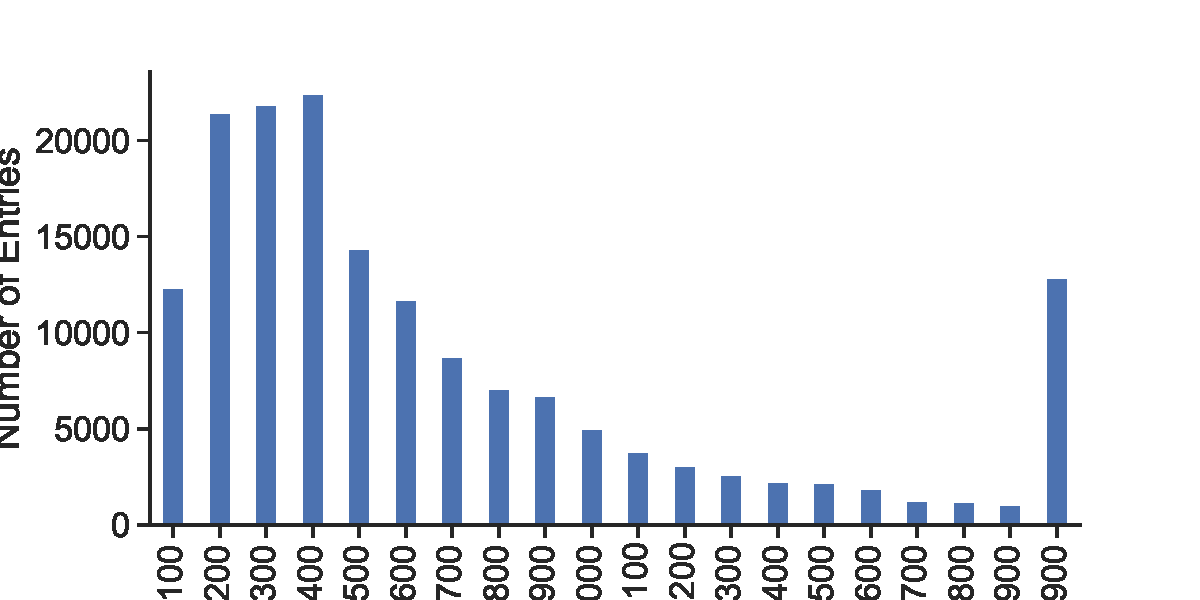
\includegraphics[width=0.45\textwidth]{paper/figures/Fig2/pdb_statistics.pdf}
        \caption{Statistics on all PDB entries based on the number of amino acid residues, with most entries found in the interval of 100-400 residues as of May 26th 2020.}
        \label{fig:pdb_stats}
\end{figure}

Protein chain lengths in the PDB vary from small fragments of less than 10 amino acids to large agglomerates of over 2000 residues. The most frequently occurring chain lengths, however are between 100 and 400 residues as shown in Fig.~\ref{fig:pdb_stats}. \red{For our analysis, we have thus chosen ............ structures of around 200, ........ structures of around 300 and .......... structures of around 400 residues from the PDB.} Those have been converted to PCN's based on the measured locations of their residues to analyze the distribution of residue distances between connected amino acids. The resulting distribution is compared to those generated in simulations in~\cite{molkenthin2020self} as well as the above derived theoretical expression. The latter, however, is scaled with a factor to account for the different dimensionality, as well as approximations made in the derivation.

The results are shown logarithmically scaled in Fig.\ref{fig:sdd}. \red{For all three lengths, the distributions show an approximate power law decay with slopes of $...\pm ...$, which is consistent with both, the simulated results ans the theoretical approximation.}

\begin{figure}[t]
        \centering
	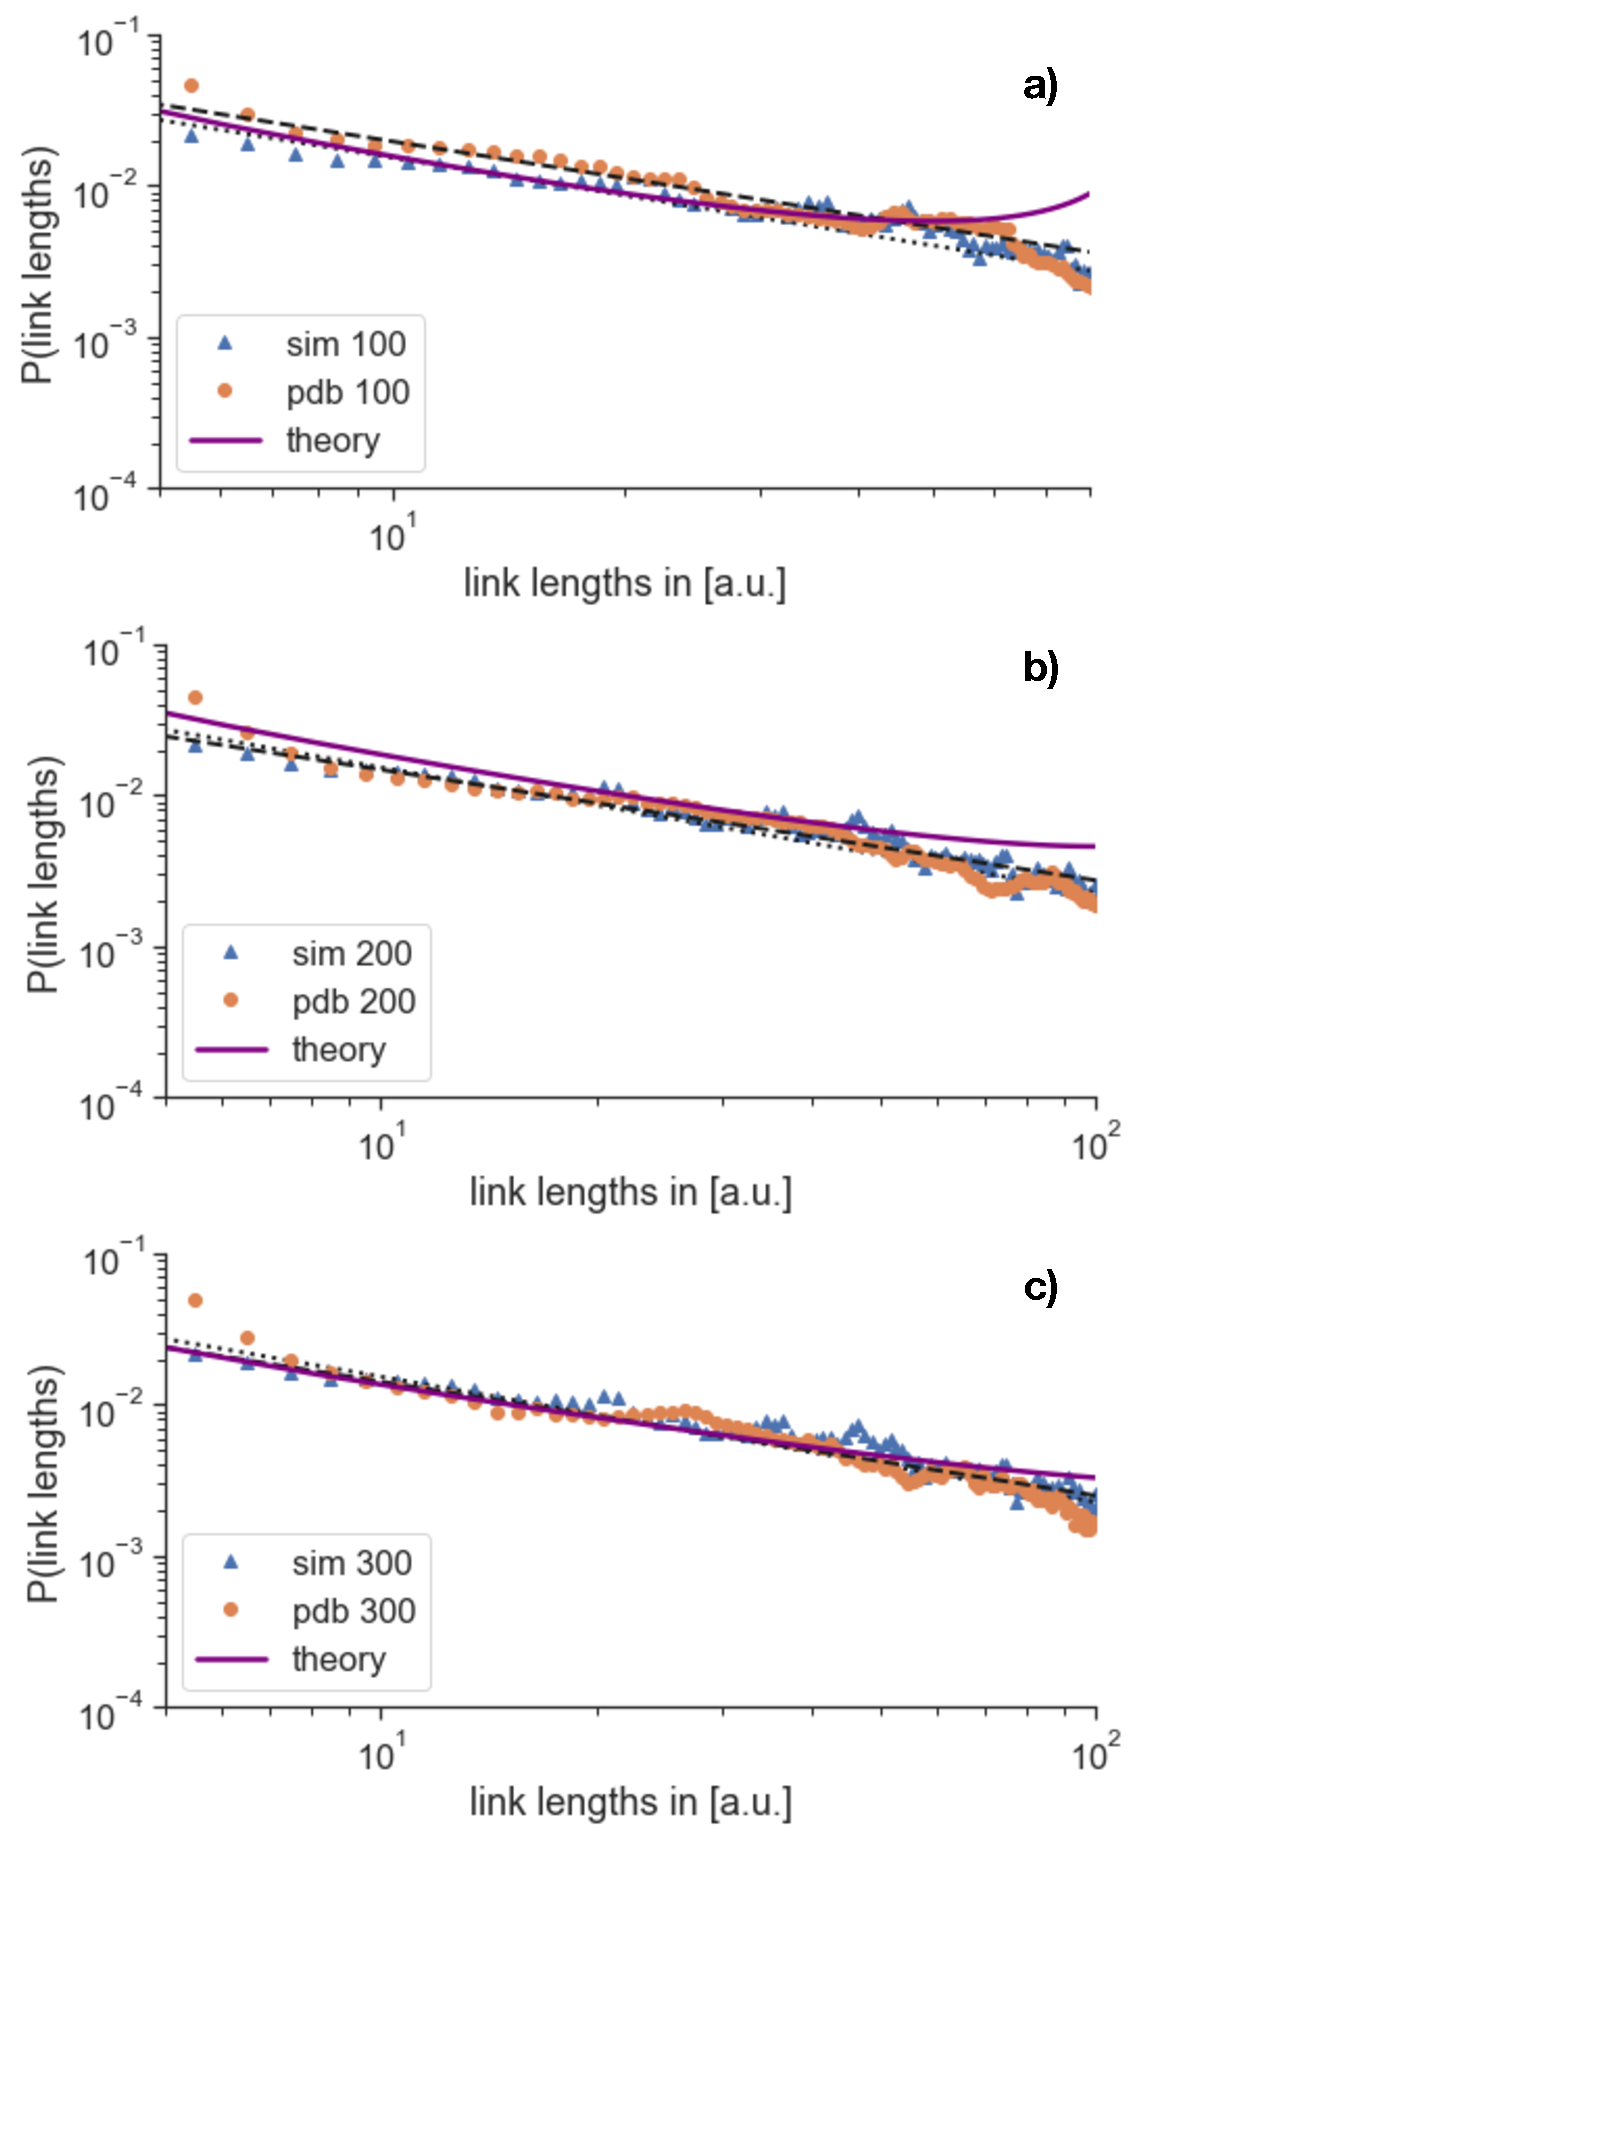
\includegraphics[width=0.45\textwidth]{paper/figures/Fig3/Fig3.pdf}
        \caption{residue distance distributions for real and simulated folds for a) Chain lengths around 200 b) chain lengths around 300 c) chain lengths around 400. \red{Depending on what this looks like when we have all the data, perhaps adding error bars could be nice. Also, since i'm mentioning the overrepresentation of separations 2 to 4, maybe those should be shown. If it fits better we can take them out for the fits and stuff.}
        }
        \label{fig:sdd}
\end{figure}

We observe that, while the general shape seems to match, in real proteins residue distances of 2 to 4 amino acids are slightly over-represented (see Fig.\ref{fig:sdd}).
The over-representation of very short residue distances is an artefact of the different network construction for simulated (and theoretically approximated) networks and PCNs. While in the simulation all links are equally long and links are made until no longer possible, the parameter, determining the connectivity in PCNs is the cutoff distance $d_c$, which is chosen such that the number of links in the PCN is comparable to those in a simulated network of the same $N$. This leads to a larger range of bond angles randomly resulting in connections for small $s$ and thus an over-representation of those links.

\section*{Conclusion}
The tertiary structures of folded proteins have long been one of the most important mysteries of Biophysics. While for individual structures, detailed molecular dynamics or statistical models are essential in approaching these questions, general statements for the ensemble of folded proteins can be made with simple models.

Here we have introduced and analyzed the residue distance $s$ and its probability distribution $P(s)$ in measured and simulated protein structures. For the equivalent model in two dimensions we have used a mean-field approach to derive an analytic approximation for the residue distance distribution, which appears to agree with the simulated and measured distributions.
We have thus demonstrated in analytical calculations as well as direct simulations how a random linking model with geometric constraints, such as the ones introduced in \cite{molkenthin2016scaling, molkenthin2020self} generates a residue distance distribution, that resembles a power-law, similar to the one found in folded proteins. This feature of protein network structure has previously been used in the heuristic model to generate protein-like structures in \cite{bartoli2008effect}.

Gaining a better understanding of the ensemble of folded protein structures can help guide the way to a better understanding of the constraints within which structures may occur. Together with an understanding of secondary structure principles, such as those in
\cite{Danielsson2010, Molkenthin2011}, this can help to narrow down the complex energy landscapes and find paths through them more effectively in the future.

\section*{Declarations}
\subsection{Availability of data and materials}
All data generated or analysed during this study are included in this published article [and its supplementary information files].
\subsection{Competing interests}
The authors declare no competing interests.
\subsection{Funding}
This research was supported by ...
\subsection{Authors' contributions}

\subsection{Acknowledgements}
We thank Marc Timme for fruitful discussions.

\bibliographystyle{unsrt}
\bibliography{proteins}

\appendix
\section{Supplemental Material Collection}
\section{Random ideas}
\begin{itemize}
    \item Why is the beginning different for simulations?
    \item Does the dip disappear for IDPs
    \item Can we use all NMR structures for IDPs
    \item Would it help using more simulated structures than just the Crystal structure. 
\end{itemize}



\end{document}